\documentclass[1p]{elsarticle_modified}
%\bibliographystyle{elsarticle-num}

%\usepackage[colorlinks]{hyperref}
%\usepackage{abbrmath_seonhwa} %\Abb, \Ascr, \Acal ,\Abf, \Afrak
\usepackage{amsfonts}
\usepackage{amssymb}
\usepackage{amsmath}
\usepackage{amsthm}
\usepackage{scalefnt}
\usepackage{amsbsy}
\usepackage{kotex}
\usepackage{caption}
\usepackage{subfig}
\usepackage{color}
\usepackage{graphicx}
\usepackage{xcolor} %% white, black, red, green, blue, cyan, magenta, yellow
\usepackage{float}
\usepackage{setspace}
\usepackage{hyperref}

\usepackage{tikz}
\usetikzlibrary{arrows}

\usepackage{multirow}
\usepackage{array} % fixed length table
\usepackage{hhline}

%%%%%%%%%%%%%%%%%%%%%
\makeatletter
\renewcommand*\env@matrix[1][\arraystretch]{%
	\edef\arraystretch{#1}%
	\hskip -\arraycolsep
	\let\@ifnextchar\new@ifnextchar
	\array{*\c@MaxMatrixCols c}}
\makeatother %https://tex.stackexchange.com/questions/14071/how-can-i-increase-the-line-spacing-in-a-matrix
%%%%%%%%%%%%%%%

\usepackage[normalem]{ulem}

\newcommand{\msout}[1]{\ifmmode\text{\sout{\ensuremath{#1}}}\else\sout{#1}\fi}
%SOURCE: \msout is \stkout macro in https://tex.stackexchange.com/questions/20609/strikeout-in-math-mode

\newcommand{\cancel}[1]{
	\ifmmode
	{\color{red}\msout{#1}}
	\else
	{\color{red}\sout{#1}}
	\fi
}

\newcommand{\add}[1]{
	{\color{blue}\uwave{#1}}
}

\newcommand{\replace}[2]{
	\ifmmode
	{\color{red}\msout{#1}}{\color{blue}\uwave{#2}}
	\else
	{\color{red}\sout{#1}}{\color{blue}\uwave{#2}}
	\fi
}

\newcommand{\Sol}{\mathcal{S}} %segment
\newcommand{\D}{D} %diagram
\newcommand{\A}{\mathcal{A}} %arc


%%%%%%%%%%%%%%%%%%%%%%%%%%%%%5 test

\def\sl{\operatorname{\textup{SL}}(2,\Cbb)}
\def\psl{\operatorname{\textup{PSL}}(2,\Cbb)}
\def\quan{\mkern 1mu \triangleright \mkern 1mu}

\theoremstyle{definition}
\newtheorem{thm}{Theorem}[section]
\newtheorem{prop}[thm]{Proposition}
\newtheorem{lem}[thm]{Lemma}
\newtheorem{ques}[thm]{Question}
\newtheorem{cor}[thm]{Corollary}
\newtheorem{defn}[thm]{Definition}
\newtheorem{exam}[thm]{Example}
\newtheorem{rmk}[thm]{Remark}
\newtheorem{alg}[thm]{Algorithm}

\newcommand{\I}{\sqrt{-1}}
\begin{document}

%\begin{frontmatter}
%
%\title{Boundary parabolic representations of knots up to 8 crossings}
%
%%% Group authors per affiliation:
%\author{Yunhi Cho} 
%\address{Department of Mathematics, University of Seoul, Seoul, Korea}
%\ead{yhcho@uos.ac.kr}
%
%
%\author{Seonhwa Kim} %\fnref{s_kim}}
%\address{Center for Geometry and Physics, Institute for Basic Science, Pohang, 37673, Korea}
%\ead{ryeona17@ibs.re.kr}
%
%\author{Hyuk Kim}
%\address{Department of Mathematical Sciences, Seoul National University, Seoul 08826, Korea}
%\ead{hyukkim@snu.ac.kr}
%
%\author{Seokbeom Yoon}
%\address{Department of Mathematical Sciences, Seoul National University, Seoul, 08826,  Korea}
%\ead{sbyoon15@snu.ac.kr}
%
%\begin{abstract}
%We find all boundary parabolic representation of knots up to 8 crossings.
%
%\end{abstract}
%\begin{keyword}
%    \MSC[2010] 57M25 
%\end{keyword}
%
%\end{frontmatter}

%\linenumbers
%\tableofcontents
%
\newcommand\colored[1]{\textcolor{white}{\rule[-0.35ex]{0.8em}{1.4ex}}\kern-0.8em\color{red} #1}%
%\newcommand\colored[1]{\textcolor{white}{ #1}\kern-2.17ex	\textcolor{white}{ #1}\kern-1.81ex	\textcolor{white}{ #1}\kern-2.15ex\color{red}#1	}

{\Large $\underline{12a_{0651}~(K12a_{0651})}$}

\setlength{\tabcolsep}{10pt}
\renewcommand{\arraystretch}{1.6}
\vspace{1cm}\begin{tabular}{m{100pt}>{\centering\arraybackslash}m{274pt}}
\multirow{5}{120pt}{
	\centering
	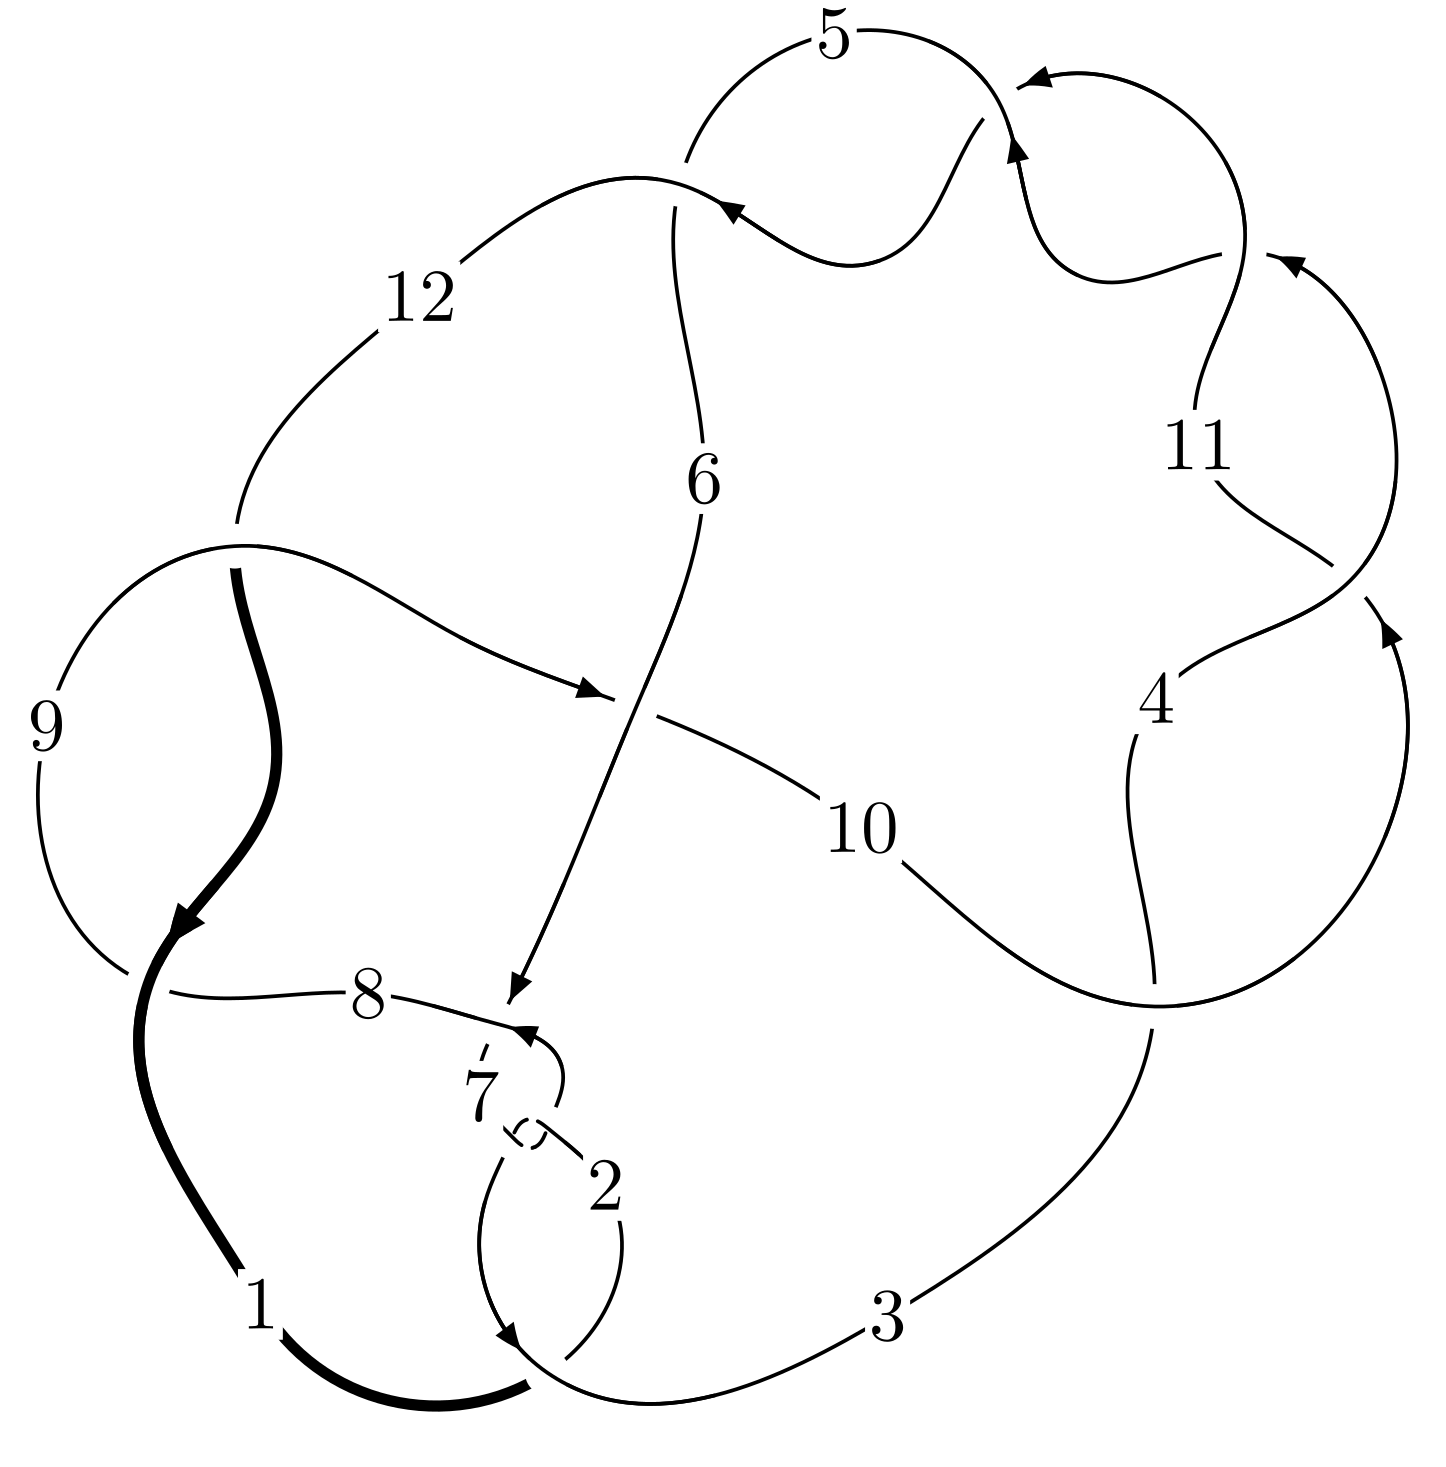
\includegraphics[width=112pt]{../../../GIT/diagram.site/Diagrams/png/1452_12a_0651.png}\\
\ \ \ A knot diagram\footnotemark}&
\allowdisplaybreaks
\textbf{Linearized knot diagam} \\
\cline{2-2}
 &
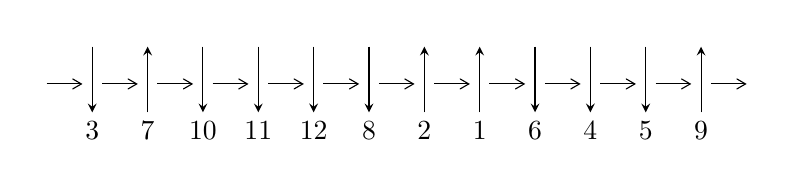
\begin{tikzpicture}[x=20pt, y=17pt]
	% nodes
	\node (C0) at (0, 0) {};
	\node (C1) at (1, 0) {};
	\node (C1U) at (1, +1) {};
	\node (C1D) at (1, -1) {3};

	\node (C2) at (2, 0) {};
	\node (C2U) at (2, +1) {};
	\node (C2D) at (2, -1) {7};

	\node (C3) at (3, 0) {};
	\node (C3U) at (3, +1) {};
	\node (C3D) at (3, -1) {10};

	\node (C4) at (4, 0) {};
	\node (C4U) at (4, +1) {};
	\node (C4D) at (4, -1) {11};

	\node (C5) at (5, 0) {};
	\node (C5U) at (5, +1) {};
	\node (C5D) at (5, -1) {12};

	\node (C6) at (6, 0) {};
	\node (C6U) at (6, +1) {};
	\node (C6D) at (6, -1) {8};

	\node (C7) at (7, 0) {};
	\node (C7U) at (7, +1) {};
	\node (C7D) at (7, -1) {2};

	\node (C8) at (8, 0) {};
	\node (C8U) at (8, +1) {};
	\node (C8D) at (8, -1) {1};

	\node (C9) at (9, 0) {};
	\node (C9U) at (9, +1) {};
	\node (C9D) at (9, -1) {6};

	\node (C10) at (10, 0) {};
	\node (C10U) at (10, +1) {};
	\node (C10D) at (10, -1) {4};

	\node (C11) at (11, 0) {};
	\node (C11U) at (11, +1) {};
	\node (C11D) at (11, -1) {5};

	\node (C12) at (12, 0) {};
	\node (C12U) at (12, +1) {};
	\node (C12D) at (12, -1) {9};
	\node (C13) at (13, 0) {};

	% arrows
	\draw[->,>={angle 60}]
	(C0) edge (C1) (C1) edge (C2) (C2) edge (C3) (C3) edge (C4) (C4) edge (C5) (C5) edge (C6) (C6) edge (C7) (C7) edge (C8) (C8) edge (C9) (C9) edge (C10) (C10) edge (C11) (C11) edge (C12) (C12) edge (C13) ;	\draw[->,>=stealth]
	(C1U) edge (C1D) (C2D) edge (C2U) (C3U) edge (C3D) (C4U) edge (C4D) (C5U) edge (C5D) (C6U) edge (C6D) (C7D) edge (C7U) (C8D) edge (C8U) (C9U) edge (C9D) (C10U) edge (C10D) (C11U) edge (C11D) (C12D) edge (C12U) ;
	\end{tikzpicture} \\
\hhline{~~} \\& 
\textbf{Solving Sequence} \\ \cline{2-2} 
 &
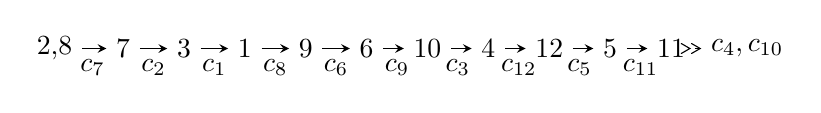
\begin{tikzpicture}[x=22pt, y=7pt]
	% node
	\node (A0) at (-1/8, 0) {2,8};
	\node (A1) at (1, 0) {7};
	\node (A2) at (2, 0) {3};
	\node (A3) at (3, 0) {1};
	\node (A4) at (4, 0) {9};
	\node (A5) at (5, 0) {6};
	\node (A6) at (6, 0) {10};
	\node (A7) at (7, 0) {4};
	\node (A8) at (8, 0) {12};
	\node (A9) at (9, 0) {5};
	\node (A10) at (10, 0) {11};
	\node (C1) at (1/2, -1) {$c_{7}$};
	\node (C2) at (3/2, -1) {$c_{2}$};
	\node (C3) at (5/2, -1) {$c_{1}$};
	\node (C4) at (7/2, -1) {$c_{8}$};
	\node (C5) at (9/2, -1) {$c_{6}$};
	\node (C6) at (11/2, -1) {$c_{9}$};
	\node (C7) at (13/2, -1) {$c_{3}$};
	\node (C8) at (15/2, -1) {$c_{12}$};
	\node (C9) at (17/2, -1) {$c_{5}$};
	\node (C10) at (19/2, -1) {$c_{11}$};
	\node (A11) at (45/4, 0) {$c_{4},c_{10}$};

	% edge
	\draw[->,>=stealth]	
	(A0) edge (A1) (A1) edge (A2) (A2) edge (A3) (A3) edge (A4) (A4) edge (A5) (A5) edge (A6) (A6) edge (A7) (A7) edge (A8) (A8) edge (A9) (A9) edge (A10) ;
	\draw[->>,>={angle 60}]	
	(A10) edge (A11);
\end{tikzpicture} \\ 

\end{tabular} \\

\footnotetext{
The image of knot diagram is generated by the software ``\textbf{Draw programme}" developed by Andrew Bartholomew(\url{http://www.layer8.co.uk/maths/draw/index.htm\#Running-draw}), where we modified some parts for our purpose(\url{https://github.com/CATsTAILs/LinksPainter}).
}\phantom \\ \newline 
\centering \textbf{Ideals for irreducible components\footnotemark of $X_{\text{par}}$} 
 
\begin{align*}
I^u_{1}&=\langle 
u^{48}- u^{47}+\cdots-2 u^2-1\rangle \\
\\
\end{align*}
\raggedright * 1 irreducible components of $\dim_{\mathbb{C}}=0$, with total 48 representations.\\
\footnotetext{All coefficients of polynomials are rational numbers. But the coefficients are sometimes approximated in decimal forms when there is not enough margin.}
\newpage
\renewcommand{\arraystretch}{1}
\centering \section*{I. $I^u_{1}= \langle u^{48}- u^{47}+\cdots-2 u^2-1 \rangle$}
\flushleft \textbf{(i) Arc colorings}\\
\begin{tabular}{m{7pt} m{180pt} m{7pt} m{180pt} }
\flushright $a_{2}=$&$\begin{pmatrix}0\\u\end{pmatrix}$ \\
\flushright $a_{8}=$&$\begin{pmatrix}1\\0\end{pmatrix}$ \\
\flushright $a_{7}=$&$\begin{pmatrix}1\\u^2\end{pmatrix}$ \\
\flushright $a_{3}=$&$\begin{pmatrix}u\\u^3+u\end{pmatrix}$ \\
\flushright $a_{1}=$&$\begin{pmatrix}u^3\\u^5+u^3+u\end{pmatrix}$ \\
\flushright $a_{9}=$&$\begin{pmatrix}- u^8- u^6- u^4+1\\- u^{10}-2 u^8-3 u^6-2 u^4- u^2\end{pmatrix}$ \\
\flushright $a_{6}=$&$\begin{pmatrix}u^2+1\\u^2\end{pmatrix}$ \\
\flushright $a_{10}=$&$\begin{pmatrix}u^{14}+3 u^{12}+6 u^{10}+7 u^8+6 u^6+4 u^4+2 u^2+1\\u^{14}+2 u^{12}+3 u^{10}+2 u^8- u^2\end{pmatrix}$ \\
\flushright $a_{4}=$&$\begin{pmatrix}- u^{31}-6 u^{29}+\cdots-18 u^5-6 u^3\\- u^{31}-5 u^{29}+\cdots+2 u^3+u\end{pmatrix}$ \\
\flushright $a_{12}=$&$\begin{pmatrix}u^{13}+2 u^{11}+3 u^9+2 u^7- u\\u^{15}+3 u^{13}+6 u^{11}+7 u^9+6 u^7+4 u^5+2 u^3+u\end{pmatrix}$ \\
\flushright $a_{5}=$&$\begin{pmatrix}- u^{30}-5 u^{28}+\cdots+2 u^2+1\\- u^{32}-6 u^{30}+\cdots-18 u^6-6 u^4\end{pmatrix}$ \\
\flushright $a_{11}=$&$\begin{pmatrix}- u^{47}-8 u^{45}+\cdots+18 u^5+6 u^3\\- u^{47}+u^{46}+\cdots-2 u^2-1\end{pmatrix}$\\&\end{tabular}
\flushleft \textbf{(ii) Obstruction class $= -1$}\\~\\
\flushleft \textbf{(iii) Cusp Shapes $= 4 u^{46}-4 u^{45}+\cdots+12 u-6$}\\~\\
\newpage\renewcommand{\arraystretch}{1}
\flushleft \textbf{(iv) u-Polynomials at the component}\newline \\
\begin{tabular}{m{50pt}|m{274pt}}
Crossings & \hspace{64pt}u-Polynomials at each crossing \\
\hline $$\begin{aligned}c_{1},c_{6}\end{aligned}$$&$\begin{aligned}
&u^{48}+17 u^{47}+\cdots+4 u+1
\end{aligned}$\\
\hline $$\begin{aligned}c_{2},c_{7}\end{aligned}$$&$\begin{aligned}
&u^{48}+u^{47}+\cdots-2 u^2-1
\end{aligned}$\\
\hline $$\begin{aligned}c_{3},c_{4},c_{5}\\c_{10},c_{11}\end{aligned}$$&$\begin{aligned}
&u^{48}- u^{47}+\cdots-2 u-1
\end{aligned}$\\
\hline $$\begin{aligned}c_{8},c_{12}\end{aligned}$$&$\begin{aligned}
&u^{48}-5 u^{47}+\cdots+100 u-39
\end{aligned}$\\
\hline $$\begin{aligned}c_{9}\end{aligned}$$&$\begin{aligned}
&u^{48}-5 u^{47}+\cdots+912 u+1305
\end{aligned}$\\
\hline
\end{tabular}\\~\\
\newpage\renewcommand{\arraystretch}{1}
\flushleft \textbf{(v) Riley Polynomials at the component}\newline \\
\begin{tabular}{m{50pt}|m{274pt}}
Crossings & \hspace{64pt}Riley Polynomials at each crossing \\
\hline $$\begin{aligned}c_{1},c_{6}\end{aligned}$$&$\begin{aligned}
&y^{48}+29 y^{47}+\cdots-16 y+1
\end{aligned}$\\
\hline $$\begin{aligned}c_{2},c_{7}\end{aligned}$$&$\begin{aligned}
&y^{48}+17 y^{47}+\cdots+4 y+1
\end{aligned}$\\
\hline $$\begin{aligned}c_{3},c_{4},c_{5}\\c_{10},c_{11}\end{aligned}$$&$\begin{aligned}
&y^{48}-63 y^{47}+\cdots+4 y+1
\end{aligned}$\\
\hline $$\begin{aligned}c_{8},c_{12}\end{aligned}$$&$\begin{aligned}
&y^{48}+37 y^{47}+\cdots+24632 y+1521
\end{aligned}$\\
\hline $$\begin{aligned}c_{9}\end{aligned}$$&$\begin{aligned}
&y^{48}-23 y^{47}+\cdots-23246424 y+1703025
\end{aligned}$\\
\hline
\end{tabular}\\~\\
\newpage\flushleft \textbf{(vi) Complex Volumes and Cusp Shapes}
$$\begin{array}{c|c|c}  
\text{Solutions to }I^u_{1}& \I (\text{vol} + \sqrt{-1}CS) & \text{Cusp shape}\\
 \hline 
\begin{aligned}
u &= \phantom{-}0.802127 + 0.589214 I\end{aligned}
 & -13.2341 - 6.6512 I & -8.69292 + 2.70499 I \\ \hline\begin{aligned}
u &= \phantom{-}0.802127 - 0.589214 I\end{aligned}
 & -13.2341 + 6.6512 I & -8.69292 - 2.70499 I \\ \hline\begin{aligned}
u &= -0.780450 + 0.595412 I\end{aligned}
 & -3.45383 + 5.14659 I & -7.86923 - 4.15340 I \\ \hline\begin{aligned}
u &= -0.780450 - 0.595412 I\end{aligned}
 & -3.45383 - 5.14659 I & -7.86923 + 4.15340 I \\ \hline\begin{aligned}
u &= -0.306787 + 0.928044 I\end{aligned}
 & -13.29560 - 2.74578 I & -13.24399 + 4.02587 I \\ \hline\begin{aligned}
u &= -0.306787 - 0.928044 I\end{aligned}
 & -13.29560 + 2.74578 I & -13.24399 - 4.02587 I \\ \hline\begin{aligned}
u &= \phantom{-}0.744340 + 0.609755 I\end{aligned}
 & \phantom{-}0.47988 - 2.41400 I & -2.77620 + 3.95017 I \\ \hline\begin{aligned}
u &= \phantom{-}0.744340 - 0.609755 I\end{aligned}
 & \phantom{-}0.47988 + 2.41400 I & -2.77620 - 3.95017 I \\ \hline\begin{aligned}
u &= -0.709694 + 0.805377 I\end{aligned}
 & \phantom{-}1.43993 - 0.10326 I & -4.11691 - 1.57301 I \\ \hline\begin{aligned}
u &= -0.709694 - 0.805377 I\end{aligned}
 & \phantom{-}1.43993 + 0.10326 I & -4.11691 + 1.57301 I \\ \hline\begin{aligned}
u &= -0.019095 + 1.077630 I\end{aligned}
 & -5.06998 - 1.60211 I & -10.45738 + 4.05120 I \\ \hline\begin{aligned}
u &= -0.019095 - 1.077630 I\end{aligned}
 & -5.06998 + 1.60211 I & -10.45738 - 4.05120 I \\ \hline\begin{aligned}
u &= \phantom{-}0.750182 + 0.779791 I\end{aligned}
 & -7.19201 - 0.77835 I & -5.36224 + 0.06889 I \\ \hline\begin{aligned}
u &= \phantom{-}0.750182 - 0.779791 I\end{aligned}
 & -7.19201 + 0.77835 I & -5.36224 - 0.06889 I \\ \hline\begin{aligned}
u &= -0.669363 + 0.604587 I\end{aligned}
 & \phantom{-}0.001527 - 0.587302 I & -4.68221 + 4.09309 I \\ \hline\begin{aligned}
u &= -0.669363 - 0.604587 I\end{aligned}
 & \phantom{-}0.001527 + 0.587302 I & -4.68221 - 4.09309 I \\ \hline\begin{aligned}
u &= \phantom{-}0.040819 + 1.103530 I\end{aligned}
 & -9.34090 + 4.19623 I & -14.8023 - 4.2142 I \\ \hline\begin{aligned}
u &= \phantom{-}0.040819 - 1.103530 I\end{aligned}
 & -9.34090 - 4.19623 I & -14.8023 + 4.2142 I \\ \hline\begin{aligned}
u &= \phantom{-}0.701243 + 0.856750 I\end{aligned}
 & \phantom{-}3.68589 + 2.68723 I & \phantom{-}1.90848 - 3.59326 I \\ \hline\begin{aligned}
u &= \phantom{-}0.701243 - 0.856750 I\end{aligned}
 & \phantom{-}3.68589 - 2.68723 I & \phantom{-}1.90848 + 3.59326 I \\ \hline\begin{aligned}
u &= \phantom{-}0.303851 + 0.826787 I\end{aligned}
 & -3.75546 + 2.27659 I & -12.89646 - 5.30128 I \\ \hline\begin{aligned}
u &= \phantom{-}0.303851 - 0.826787 I\end{aligned}
 & -3.75546 - 2.27659 I & -12.89646 + 5.30128 I \\ \hline\begin{aligned}
u &= -0.050388 + 1.121400 I\end{aligned}
 & -19.3092 - 5.5995 I & -15.3152 + 3.0524 I \\ \hline\begin{aligned}
u &= -0.050388 - 1.121400 I\end{aligned}
 & -19.3092 + 5.5995 I & -15.3152 - 3.0524 I \\ \hline\begin{aligned}
u &= -0.701027 + 0.900492 I\end{aligned}
 & \phantom{-}1.15320 - 5.29793 I & -5.03627 + 7.68449 I \\ \hline\begin{aligned}
u &= -0.701027 - 0.900492 I\end{aligned}
 & \phantom{-}1.15320 + 5.29793 I & -5.03627 - 7.68449 I \\ \hline\begin{aligned}
u &= -0.715058 + 0.438137 I\end{aligned}
 & -14.1380 - 3.7995 I & -9.38326 + 2.79474 I \\ \hline\begin{aligned}
u &= -0.715058 - 0.438137 I\end{aligned}
 & -14.1380 + 3.7995 I & -9.38326 - 2.79474 I \\ \hline\begin{aligned}
u &= \phantom{-}0.719743 + 0.928582 I\end{aligned}
 & -7.64175 + 6.35454 I & -6.48748 - 5.77861 I \\ \hline\begin{aligned}
u &= \phantom{-}0.719743 - 0.928582 I\end{aligned}
 & -7.64175 - 6.35454 I & -6.48748 + 5.77861 I\\
 \hline 
 \end{array}$$\newpage$$\begin{array}{c|c|c}  
\text{Solutions to }I^u_{1}& \I (\text{vol} + \sqrt{-1}CS) & \text{Cusp shape}\\
 \hline 
\begin{aligned}
u &= \phantom{-}0.672923 + 0.473750 I\end{aligned}
 & -4.26296 + 2.63953 I & -9.04168 - 4.04694 I \\ \hline\begin{aligned}
u &= \phantom{-}0.672923 - 0.473750 I\end{aligned}
 & -4.26296 - 2.63953 I & -9.04168 + 4.04694 I \\ \hline\begin{aligned}
u &= \phantom{-}0.620090 + 1.027290 I\end{aligned}
 & -5.75948 + 2.34942 I & -11.55550 - 1.52820 I \\ \hline\begin{aligned}
u &= \phantom{-}0.620090 - 1.027290 I\end{aligned}
 & -5.75948 - 2.34942 I & -11.55550 + 1.52820 I \\ \hline\begin{aligned}
u &= -0.648633 + 1.012460 I\end{aligned}
 & -1.18407 - 4.57916 I & -6.64611 + 1.38024 I \\ \hline\begin{aligned}
u &= -0.648633 - 1.012460 I\end{aligned}
 & -1.18407 + 4.57916 I & -6.64611 - 1.38024 I \\ \hline\begin{aligned}
u &= -0.608868 + 1.044010 I\end{aligned}
 & -15.8277 - 1.2103 I & -12.22073 + 2.35699 I \\ \hline\begin{aligned}
u &= -0.608868 - 1.044010 I\end{aligned}
 & -15.8277 + 1.2103 I & -12.22073 - 2.35699 I \\ \hline\begin{aligned}
u &= \phantom{-}0.668938 + 1.023950 I\end{aligned}
 & -0.74329 + 7.81387 I & -4.00000 - 8.53366 I \\ \hline\begin{aligned}
u &= \phantom{-}0.668938 - 1.023950 I\end{aligned}
 & -0.74329 - 7.81387 I & -4.00000 + 8.53366 I \\ \hline\begin{aligned}
u &= -0.676813 + 1.038570 I\end{aligned}
 & -4.76998 - 10.66020 I & -9.85701 + 8.71110 I \\ \hline\begin{aligned}
u &= -0.676813 - 1.038570 I\end{aligned}
 & -4.76998 + 10.66020 I & -9.85701 - 8.71110 I \\ \hline\begin{aligned}
u &= \phantom{-}0.681817 + 1.047990 I\end{aligned}
 & -14.6043 + 12.2368 I & -10.70547 - 7.24531 I \\ \hline\begin{aligned}
u &= \phantom{-}0.681817 - 1.047990 I\end{aligned}
 & -14.6043 - 12.2368 I & -10.70547 + 7.24531 I \\ \hline\begin{aligned}
u &= -0.545430\phantom{ +0.000000I}\end{aligned}
 & -10.6248\phantom{ +0.000000I} & -6.00350\phantom{ +0.000000I} \\ \hline\begin{aligned}
u &= -0.257194 + 0.480005 I\end{aligned}
 & -0.181190 - 0.868139 I & -4.26608 + 7.69273 I \\ \hline\begin{aligned}
u &= -0.257194 - 0.480005 I\end{aligned}
 & -0.181190 + 0.868139 I & -4.26608 - 7.69273 I \\ \hline\begin{aligned}
u &= \phantom{-}0.420030\phantom{ +0.000000I}\end{aligned}
 & -1.58694\phantom{ +0.000000I} & -4.88980\phantom{ +0.000000I}\\
 \hline 
 \end{array}$$\newpage
\newpage\renewcommand{\arraystretch}{1}
\centering \section*{ II. u-Polynomials}
\begin{tabular}{m{50pt}|m{274pt}}
Crossings & \hspace{64pt}u-Polynomials at each crossing \\
\hline $$\begin{aligned}c_{1},c_{6}\end{aligned}$$&$\begin{aligned}
&u^{48}+17 u^{47}+\cdots+4 u+1
\end{aligned}$\\
\hline $$\begin{aligned}c_{2},c_{7}\end{aligned}$$&$\begin{aligned}
&u^{48}+u^{47}+\cdots-2 u^2-1
\end{aligned}$\\
\hline $$\begin{aligned}c_{3},c_{4},c_{5}\\c_{10},c_{11}\end{aligned}$$&$\begin{aligned}
&u^{48}- u^{47}+\cdots-2 u-1
\end{aligned}$\\
\hline $$\begin{aligned}c_{8},c_{12}\end{aligned}$$&$\begin{aligned}
&u^{48}-5 u^{47}+\cdots+100 u-39
\end{aligned}$\\
\hline $$\begin{aligned}c_{9}\end{aligned}$$&$\begin{aligned}
&u^{48}-5 u^{47}+\cdots+912 u+1305
\end{aligned}$\\
\hline
\end{tabular}\newpage\renewcommand{\arraystretch}{1}
\centering \section*{ III. Riley Polynomials}
\begin{tabular}{m{50pt}|m{274pt}}
Crossings & \hspace{64pt}Riley Polynomials at each crossing \\
\hline $$\begin{aligned}c_{1},c_{6}\end{aligned}$$&$\begin{aligned}
&y^{48}+29 y^{47}+\cdots-16 y+1
\end{aligned}$\\
\hline $$\begin{aligned}c_{2},c_{7}\end{aligned}$$&$\begin{aligned}
&y^{48}+17 y^{47}+\cdots+4 y+1
\end{aligned}$\\
\hline $$\begin{aligned}c_{3},c_{4},c_{5}\\c_{10},c_{11}\end{aligned}$$&$\begin{aligned}
&y^{48}-63 y^{47}+\cdots+4 y+1
\end{aligned}$\\
\hline $$\begin{aligned}c_{8},c_{12}\end{aligned}$$&$\begin{aligned}
&y^{48}+37 y^{47}+\cdots+24632 y+1521
\end{aligned}$\\
\hline $$\begin{aligned}c_{9}\end{aligned}$$&$\begin{aligned}
&y^{48}-23 y^{47}+\cdots-23246424 y+1703025
\end{aligned}$\\
\hline
\end{tabular}
\vskip 2pc
\end{document}